\chapter{基于CAE-CNN的无线信号调制识别}
\section{引言}
最近,无线通信领域的研究人员已经开始将深度神经网络应用于认知无线电,并取得了一些成果[13] [12][10]。然而,他们大多是利用传统的。。。文章。。。。文章。。。\par

本章对通信信号中的无线信号调制识别问题,提出了一种基于卷积自编码器(CAE)与卷积神经网络(CNN)融合的无线信号调制识别的框架,并将此框架下的识别准确率与传统的基于特征的识别方法进行比较。

我们专注于使用两种形式的卷积神经网络来学习原始采样无线电信号时间序列示例的稀疏表示。我们利用RadioML16.04 [15]标记的无线电调制数据集进行11种调制,其中包括白噪声,振荡器漂移,采样时钟漂移和衰落的影响。这个数据集的例子如图1所示。A.纯粹无监督的稀疏表示在没有使用类标签的情况下,我们采用纯粹无监督的方法来学习数据集的稀疏表示。这可以通过应用基于依赖关系的降维技术(例如主成分分析(PCA)或独立分量分析(ICA))来完成,然而相反,我们利用输入信号的重构通过稀疏表示在自编码器神经网络中学习的一组卷积基函数[3]。自动编码器是无监督的学习构造,其中神经网络的优化目标是通过一些更有约束的维度的中间表示来最小化输出处的重构误差以匹配输入,通常使用均方误差(MSE)损失函数并且将随机梯度下降的形式用作求解器,通过从该损失项向后传播梯度以找到接近等式III-A中的最佳网络参数。我们使用RMSProp [11]和Adam [12]梯度下降求解器进行优化,两者都获得了相似的结果。\par


\section{无线传播模型}

\subsection{信道建模}
这可以被看作是一个N类的决策问题,其中我们的输入是一个复杂的基带时间序列表示接收到的信号。
也就是说,我们以离散时间步长对无线电信号的同相和正交分量进行采样,
通过大致以感兴趣的载波为中心的载波频率进行模数转换,以获得1×N的复数值向量。
典型地,这写成如等式1,其中$s(t)$是连续信号或一系列离散比特的时间序列信号,
调制到具有变化的频率,相位,振幅,轨迹或多个置换的正弦波它们。
 $c$是信号上的一些路径损耗或恒定增益项,$n(t)$是反映热噪声的加性高斯白噪声过程。
\begin{equation}\label{sec:eqt_1}
r(t) = s(t)*c + n(t)
\end{equation}
从分析的角度来看,这个简化的表达式在专家特征和决策统计的发展中被广泛使用,
但是在许多系统中,现实世界的关系看起来更像方程 \ref{sec:eqt_1} 中给出的关系。\par
\begin{equation}
	r(t) = e^{j*n_{Lo}(t)} \int_{\tau=0}^{\tau_{0}} s(n_{Clk}(t-\tau))h(\tau) + n_{Add}(t)
\end{equation}
这考虑了许多对于模型来说是非平凡的现实世界效应:通过残余载波随机游走过程调制$n_{Lo}(t)$,通过残余时钟振荡器随机游走进行重新采样,$n_{Clk}(t)$,具有时间的卷积 变化的非恒定振幅信道脉冲响应$h(t-\tau)$,以及可能不是白色的噪声相加$n_{Add}(t)$。 每个呈现一个未知的时间变化的错误来源。\par



\section{调制信号的稀疏表示}


\subsection{数据集可视化}
从时间(图1)和频域(图2)中的每一类调制中检查一个例子,我们可以看到调制之间的许多相似和差异,但是由于脉冲整形,失真和其他通道效应, 都由视觉上的人类专家容易识别。在频域中,每一个信号都遵循一个类似的带限功率包络,其形状为调制提供了一些线索,但是对于人类专家来说,为视觉判断提供了一个困难的嘈杂任务。\par
\begin{figure}[!h]
	\centering
	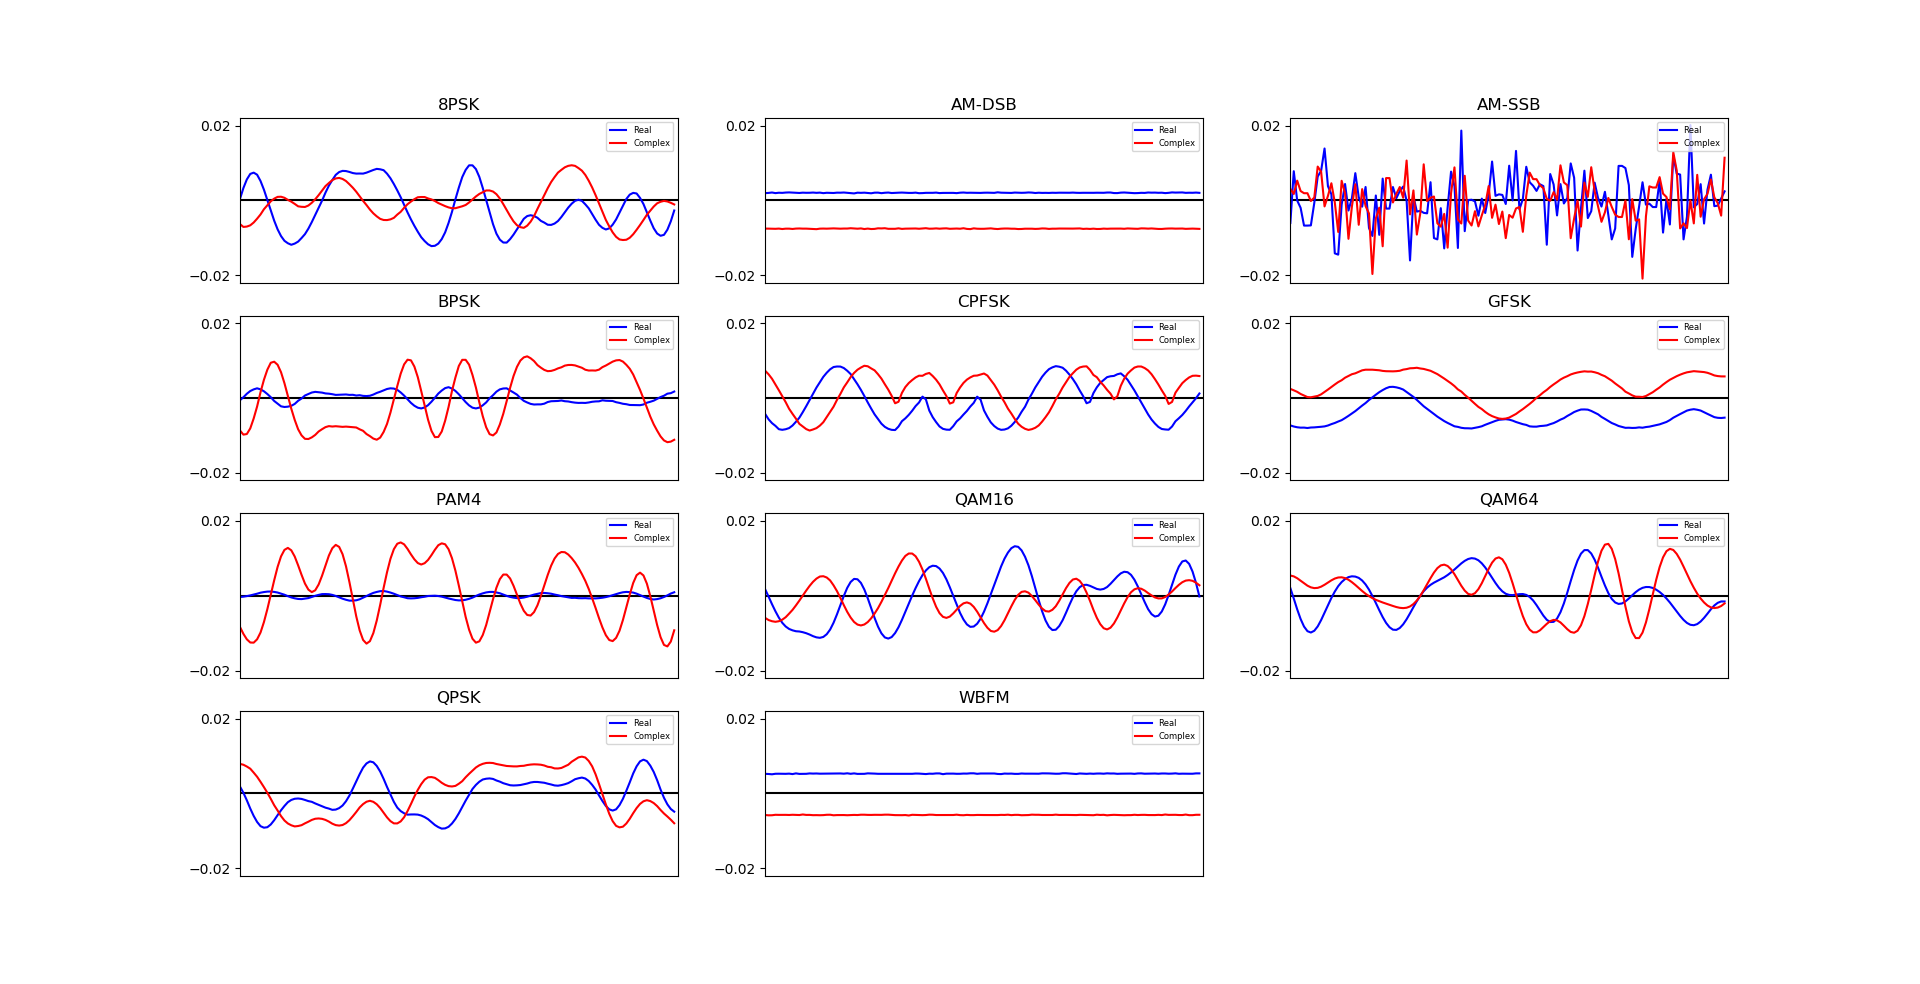
\includegraphics[scale=0.9]{figures/chapter_3/signal_view_1}
	\caption{sigmoid函数与tanh函数}\label{fig_2_2}
\end{figure}
\begin{figure}[!h]
	\centering
	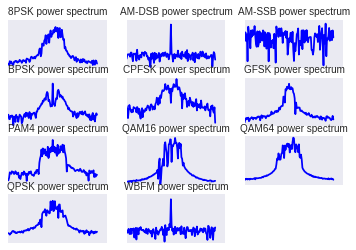
\includegraphics[scale=0.9]{figures/chapter_3/signal_view_2}
	\caption{sigmoid函数与tanh函数}\label{fig_2_2}
\end{figure}

\subsection{无监督表示学习}
纯粹无监督的稀疏表示在没有使用类标签的情况下,我们采用纯粹无监督的方法来学习数据集的稀疏表示。这可以通过应用基于依赖性的降维技术(例如主成分分析(PCA)或独立分量分析(ICA))来完成,但是相反,我们利用通过在输入信号上重构稀疏表示而给出的非线性降维在自编码器神经网络中学习的一组卷积基函数[3]。自动编码器是无监督的学习构造,其中神经网络的优化目标是通过一些更有约束的维度的中间表示来最小化输出处的重构误差以匹配输入,通常使用均方误差(MSE)损失函数并且将随机梯度下降的形式用作求解器,通过从该损失项向后传播梯度以找到接近等式III-A中的最佳网络参数。我们使用RMSProp [11]和Adam [12]梯度下降求解器进行优化,两者都获得了相似的结果。\par
通过约束网络中的中间层宽度,从而可以以低误差重建原始全维例子,通过提取用于聚类的中间稀疏编码来获得非线性降维。在这种情况下,使用类似的基函数和脉冲形状的调制可以由类似形状的卷积滤波器和编码器和解码器内的中间特征映射来表示,从而导致它们存在于该压缩空间的相似区域中。自编码器中的卷积层由于它们在时间上的不变表示性质以及受约束的参数搜索空间相对于它们的完全连接层等价物而非常适合于无线电时间序列信号表示。我们使用丢失[13]和输入噪声[7]作为正则化技术来帮助改善我们在数据集上学习表示的泛化。图2显示了我们的卷积自动编码器使用的体系结构。\par
\begin{figure}[!h]
	\centering
	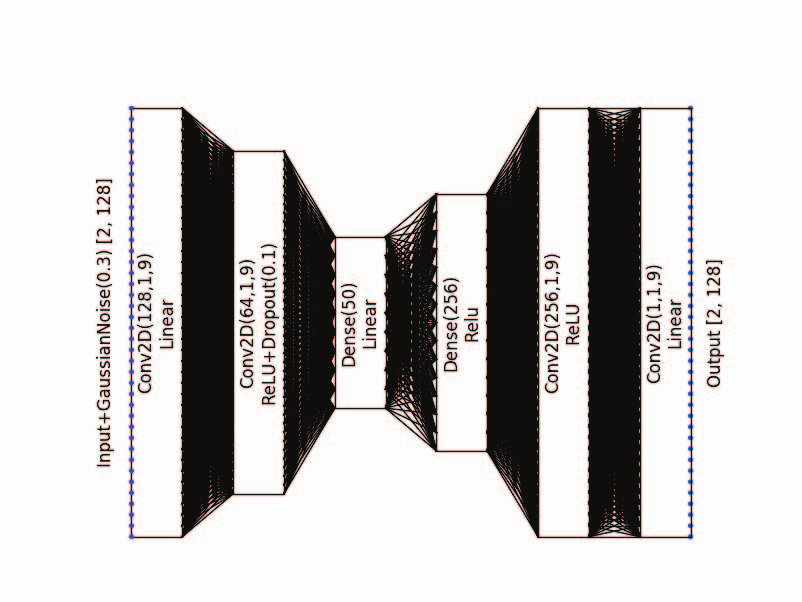
\includegraphics[scale=0.3]{figures/chapter_3/CAE}
	\caption{自编码器}	\label{fig_3_2}
\end{figure}
在自编码器的训练过程中,我们尽量减少重构均方误差(MSE),但由于我们的主要目标是获得一个良好的聚类稀疏表示,我们显着限制隐藏层维度到一个点,我们的重构作出一些可见的简化假设,偏袒在最优重构误差下降低了隐层维数。图3显示了两个训练样例,2x128输入向量的样子,1x30稀疏表示的样子,以及2x128输出重构的样子。这给了这个网络的学习代表能力的一些直觉。\par
\begin{figure}[!h]
	\centering
	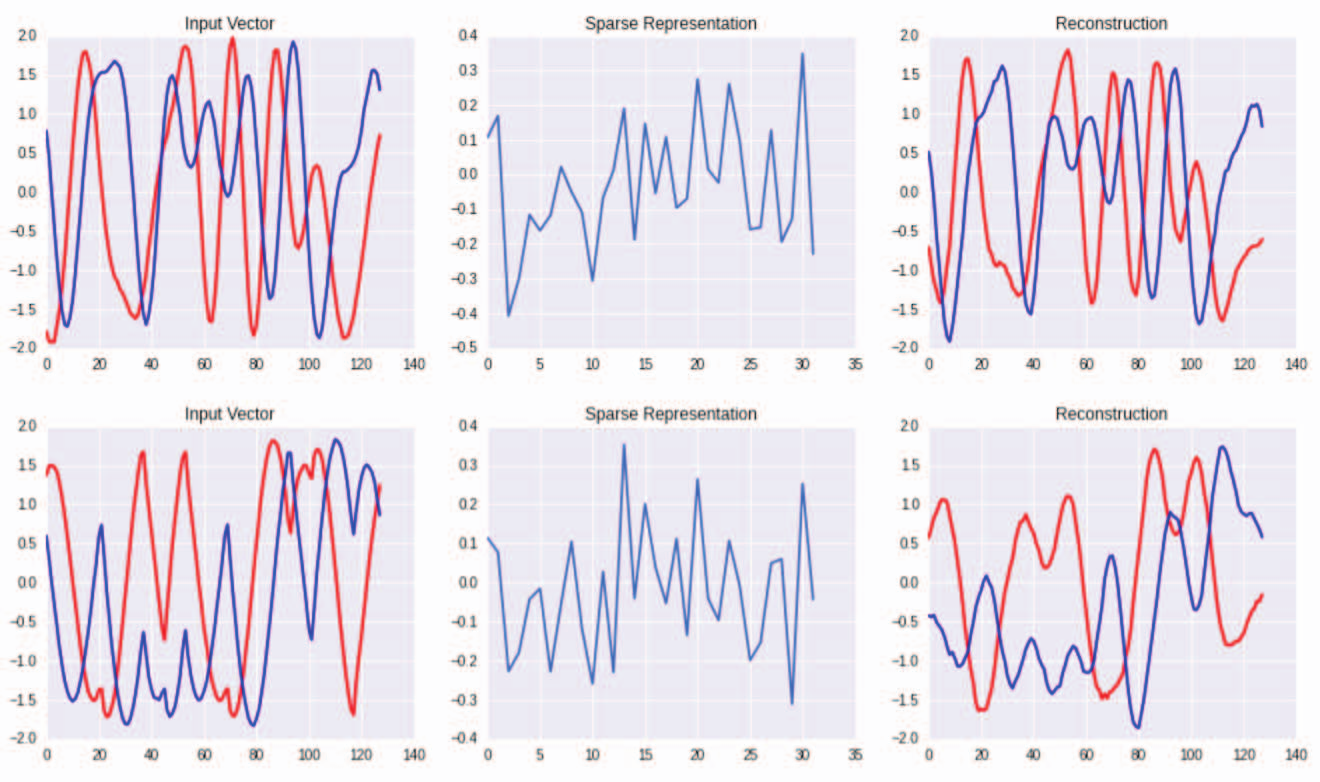
\includegraphics[scale=0.2]{figures/chapter_3/examples_cae}
	\caption{自编码器}	\label{fig_3_2}
\end{figure}
\begin{figure}[!h]
	\centering
	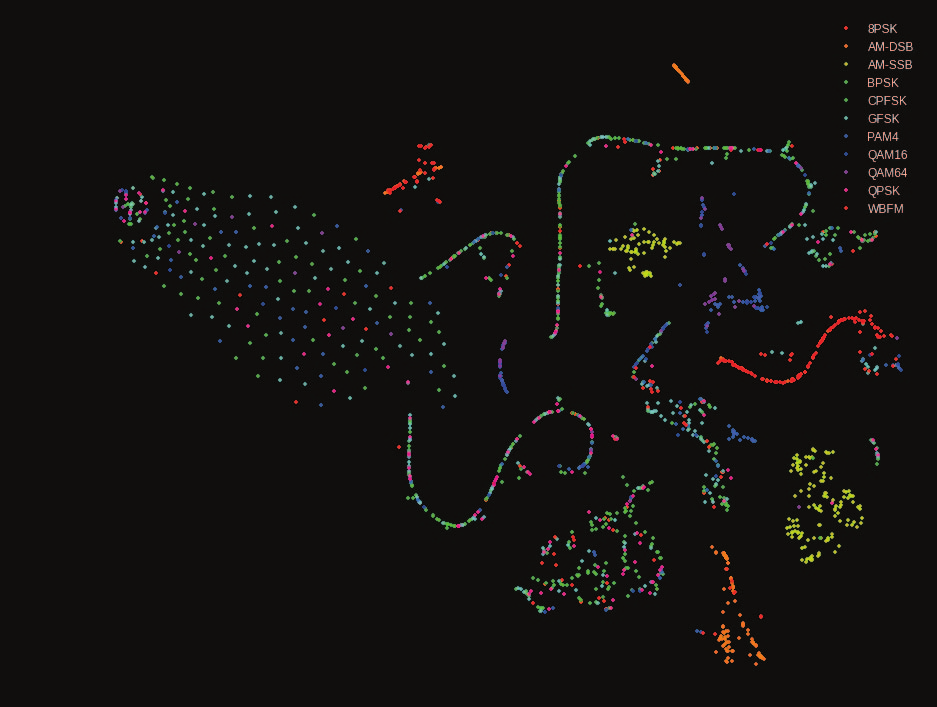
\includegraphics[scale=0.2]{figures/chapter_3/cae_fea}
	\caption{自编码器}	\label{fig_3_2}
\end{figure}

\subsection{监督引导稀疏表示}
在我们确实有一些熟练的标记数据的情况下,我们也可以使用监督训练期间学习到的判别特征生成一个稀疏表示空间。在之前的工作[14]中,我们以纯监督的方式训练卷积神经网络来标记示例,但是在这里,我们利用这个训练好的网络,放弃最后的softmax层,只保留高层学习的特征映射为稀疏表示。图4中显示了使用学习的特征映射进行有监督训练和稀疏表示提取的网络。\par
以这种方式形成的特征利用和提取可用的专业策划标签,但是在许多情况下,它们也推广并提供了在没有类别标签的特征空间中分隔额外类别的能力。因此,我们将其视为一种以监督方式进行稀疏特征学习的引导方法,并推广到包含额外的未标记训练数据的大型数据集上的半监督式识别。\par
\begin{figure}[!h]
	\centering
	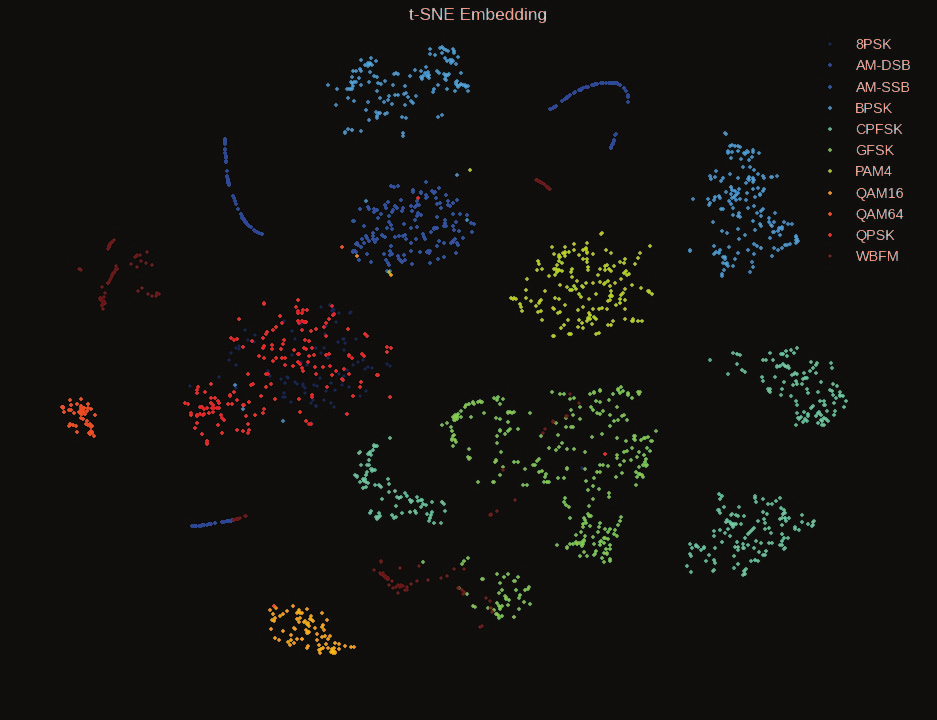
\includegraphics[scale=0.2]{figures/chapter_3/surprised_fea}
	\caption{自编码器}	\label{fig_3_2}
\end{figure}
IV。 V等同于每一种类型的消息\par
为了使这些学习表示和它们的类可分性可视化,我们在压缩的表示上执行t分布的随机相邻嵌入(t-SNE)[6],以在二维流形上显示示例,其中我们可以获得关于聚类和距离存在于底层数据集中。\par
我们首先从自编码器的表征特征空间中的类的t-SNE嵌入中看出类的聚类和可分性,如图5和6所示。在这种情况下,我们看到几个类如WBFM,AM- DSB,AM-SSB和QPSK(在ConvAE1中)已经形成了独特的,大部分可分离的簇,而其他类则表现出明显更多的混合,并且将难以通过聚类方法分离。不过这还不错,考虑到这些特征从来没有被训练成为鉴别者,但我们已经获得了一定程度的类别可分离性。我们认为对于剩余类别的可分性,或者在无监督聚类学习和可分类聚类的区分特征映射学习之间进行一定程度的迭代可能会有所帮助,但这超出了本文的研究范围。\par
其次,我们看看图7中所示的自举判别特征表示的t-SNE嵌入的聚类。在这种情况下,我们获得几乎每个调制的几乎完全可分的聚类数据集。当然,这里我们有犯有类别识别知识,当形成这个特征地图表示(在监督训练期间),但理想地这些是有区别的特征将继续推广到大量的类,并帮助区分额外的未知信号。\par


\section{基于CAE-CNN的无线信号调制识别}
我们训练几个候选神经网络。利用两个卷积层和两个密集的完全连接层(CNN和CNN2)的4层网络。除了单热输出层上的Softmax激活之外,层使用整流线性(ReLU)激活功能。我们使用这个网络深度,因为它大致相当于在MNIST等视觉领域中类似的简单数据集上运行良好的网络。\par 

\subsection{CAE-CNN算法}
正则化用于防止过度拟合。 CNN使用Dropout,卷积层权重上的kW k 2范数惩罚,鼓励最小能量基,以及第一密集层激活上的khk 1范数惩罚来鼓励解的稀疏性[5] [10]。 CNN2只使用丢失,而DNN只使用丢失。使用分类交叉熵损失函数和Adam [15]求解器进行训练,似乎在我们的数据集上略胜过RMSProp [12]。我们在Keras [16]上运行在TensorFlow [19]上的网络训练和预测,在DIGITS Devbox上的NVIDIA Cuda [8]启用的Titan X GPU上运行。图3显示了CNN架构的一个例子.CNN2是相同的但是较大的,在层1和层2中包含256和80个过滤器,在层3中包含256个神经元。评估的DNN包含4个密度层,大小分别为512,256,128 ,和n级神经元。\par

\subsection{CAE-CNN网络架构}
\begin{figure}[!h]
	\centering
	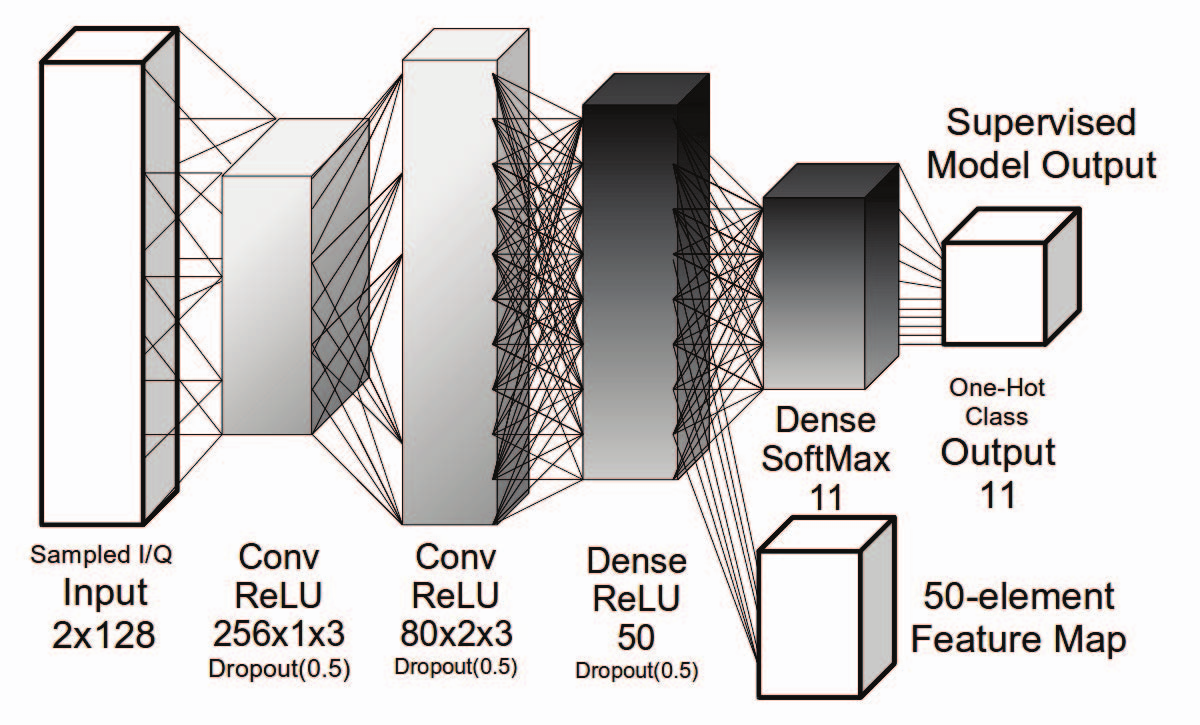
\includegraphics[scale=0.3]{figures/chapter_3/cae_cnn_frame}
	\caption{自编码器}	\label{fig_3_2}
\end{figure}

\subsection{学习复杂度}
我们使用Adam求解器训练了大约23分钟的最高复杂度模型,批量大小为1024的样本训练集大约需要15秒。我们确实观察到一些过度拟合,尽管没有正规化,但验证损失确实 没有显着变化,我们保持最佳的验证损失模型进行评估。\par
4.4 学习功能 \par
绘制学习的特征有时可以让我们直觉了解网络正在学习的底层表示。 在这种情况下,我们在下面绘制卷积层1和卷积层2的滤波器权重。 在图5中,第一层,我们有64个1x3的过滤器。 在这种情况下,我们只需获得一组边缘和梯度检测器,它们在每个I和Q通道上进行操作。\par

在卷积层2中,如图6所示的权重,我们将这个第一层特征图组合成64×16×2×3较大的特征图,其包括在I和Q通道上同时出现的情况。 这些特征图与在包括2D学习边缘检测器和Gabor滤波器的图像转换网络的较低层处所看到的特征图看起来没有太大的不同。\par


\section{结果及分析}

\subsection{分类准确率与鲁棒性}
为了评估分类器的性能,我们看一下测试数据集的分类性能。我们训练了一个包含11个调制模块的大约1200万个复杂样本的语料库。这些分为128个样本的训练样本。我们使用大约96,000个示例进行培训,并使用64,000个示例进行测试和验证。 这些样本均匀分布在从-20dB到+ 20dB的SNR中,并被标记以便我们可以评估特定子集上的性能。\par
\begin{figure}[!h]
	\centering
	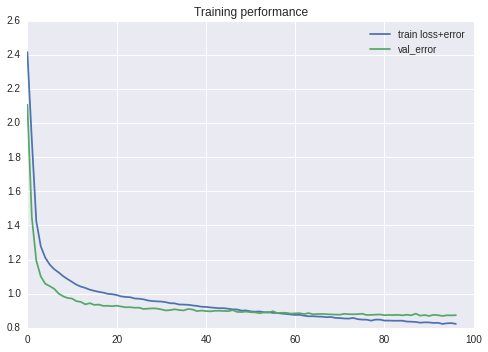
\includegraphics[scale=0.3]{figures/chapter_3/loss}
	\caption{自编码器}	\label{fig_3_2}
\end{figure}

\subsection{训练效率以及分类效率}
在训练之后,我们在测试数据集上的所有信噪比之间的分类准确率大致达到了87.4%,但要理解这个意义,我们必须检查这个分类精度如何在不同训练样本的SNR值之间进行分解,以及 它与现有的基于专家特征的分类器的性能进行比较。绘制测试集调制分类精度,作为每个分类器的示例信噪比的函数7。 实线表示直接在无线电时间序列数据上进行深度特征学习训练的分类器,而虚线表示使用前面描述的专家特征作为输入的分类器。 这种观点是检验结果的关键方法,因为在低信噪比影响范围和覆盖范围的性能,我们可以有效地使用分类器。 我们从具有大量丢失正则化(0.6)的大卷积神经网络(CNN2)中获得显着更好的低SNR分类准确性性能。 在低信噪比情况下,最佳CNN模型的性能比基于专家特征的系统的信噪比高2.5-5dB,而+ 5dB SNR性能相似。 这是一个显着的性能改进,可能至少是传感系统有效覆盖面积的两倍。\par
\begin{figure}[!h]
	\centering
	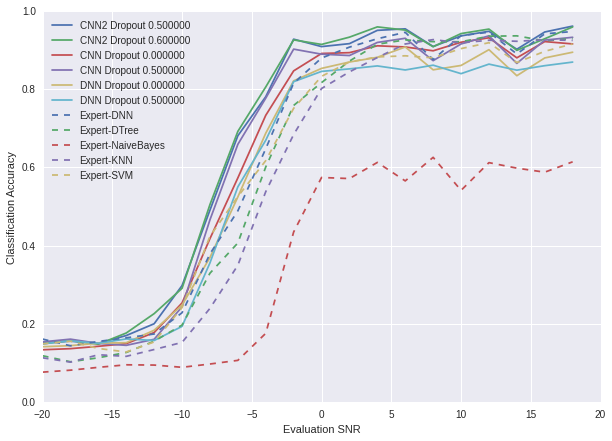
\includegraphics[scale=0.3]{figures/chapter_3/result}
	\caption{自编码器}	\label{fig_3_2}
\end{figure}
对于我们最高的SNR情况下的CNN2(0.6)分类,我们在图8中显示了一个混淆矩阵。在+18dBSNR时,在混淆矩阵中我们有一个干净的对角线,可以看到我们剩下的差异是8PSK误分类为QPSK,WBFM误分类作为AM-DSB。这两个都可以在基础数据集中解释。由于QPSK星座点由8PSK点跨越,所以包含特定比特的8PSK符号从QPSK难以分辨。在WBFM /AM-DSB的情况下,模拟语音信号具有只有载波音调存在的静默时段,这使得这些示例不可见。因此,即使在这个数据集的高信噪比下,也不可能获得100%的准确度,并使得重新合理的混淆被合理地容忍。\par

为了更好地理解性能如何随信噪比而变化,我们检查了不同信噪比级别的几个分类器的混淆矩阵。\par

在非常低的信噪比(-6dB)的情况下,在图9,10,11和12中,我们看到一个有趣的情况,其中±20%内的所有精度都在50%左右。在这种情况下,CNN2分类器上的清洁器对角线比其他3种情况显着更明显,在这个区域学习到的特征具有显着的性能优势。\par

现在,所有4个分类器的信噪比(0dB)略高但仍然很低,现在有一个明确的对角线,但是我们发现在8PSK情况下发生的非对角线误分类更少。\par

6 模型复杂性\par

许多无线电系统中的一个重要考虑因素是训练和分类运行时间,由于计算复杂性。 深度学习的一个普遍批评是对大量计算资源的需求,然而在本文中,我们的网络相对紧凑,数据集相对较小。 我们比较下面每个模型的训练和分类运行时间。 在图17中我们可以看到,我们的CNN模型确实需要大量的训练时间,但是比SVM训练案例所需要的时间要少。\par
\begin{figure}[!h]
	\centering
	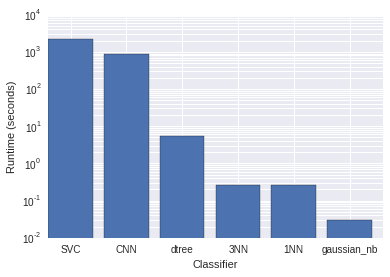
\includegraphics[scale=0.5]{figures/chapter_3/train_time}
	\caption{自编码器}	\label{fig_3_2}
\end{figure}
\begin{figure}[!h]
	\centering
	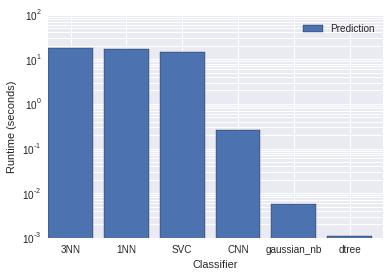
\includegraphics[scale=0.5]{figures/chapter_3/classify_time}
	\caption{自编码器}	\label{fig_3_2}
\end{figure}

在图18中显示,使用Keras编译python的这个模型的分类时间比使用scikit-learn的最近邻和SVM模型的大多数其他模型显着更快。只有决策树和GaussianNB模型获得更快的分类运行时间。在这两种情况下,基于ConvNet的这种规模的这种数据集分类模型提出了一个有吸引力的选择这个任务时,分类性能考虑。\par


通过约束网络中的中间层宽度,从而可以以低误差重建原始全维例子,通过提取用于聚类的中间稀疏编码来获得非线性降维。在这种情况下,使用类似的基函数和脉冲形状的调制可以由类似形状的卷积滤波器和编码器和解码器内的中间特征映射来表示,使得它们存在于该压缩空间的相似区域中。自编码器中的卷积层由于它们在时间上的不变表示性质以及受约束的参数搜索空间相对于它们的完全连接层等价物而非常适合于无线电时间序列信号表示。我们使用丢失[13]和输入噪声[7]作为正则化技术来帮助改善我们在数据集上学习表示的泛化。图2显示了我们的卷积自动编码器使用的体系结构。\par

\section{本章小结}

虽然这些结果并不是现有的最好的基于专家特征的调制分类器的全面比较,但是它们证明了,与相对专业的被认为的方法相比,时间序列无线电信号数据上的盲卷积网络是可行的并且工作得很好。在图7中,我们比较了几种分类器策略的准确性和信噪比,并且认为对于低信噪比和短时间的示例(128个复杂采样),这代表了调制分类的最先进的精确度方法。这种方法有可能容易地扩展到额外的调制类别,并且应该被视为依赖于无线电发射器的稳健的低SNR分类的DSA和CR系统的有力候选。\par

我们的结果与当前最好的专家系统方法的合理近似相比较,但是由于在无线电领域新兴的机器学习领域不存在强大的竞争数据集,所以很难直接比较性能和当前的现有技术状态。我们希望在以后的工作中进一步评估这一点,并将特征学习和专家方法从目前的水平上进行改进。 CNN2网络体系结构上的性能改进是不可避免的,我们花费了一些努力来优化它,但并没有做到这一点。较大的过滤器,不同的体系结构和池化层可能会显着影响性能,但是在这项工作中没有充分考虑其适用性。许多附加技术可以应用于这个问题,包括引入附加通道引起的效应的不变性,例如膨胀,I / Q不平衡,相位偏移等等。空间变换网络[17]已经证明了学习图像数据的这种不变性的强大能力,并且可以作为一个有趣的候选者,使得能够改善对这些效应的不变性学习。序列模型和递归层[13]可能能够表示信号序列嵌入,并且在更长时间表示中几乎肯定会证明是有价值的,但是我们还没有完全调查这个区域。这个应用领域已经成熟,可以进一步研究和应用,这将大大影响无线信号处理和认知无线电领域的技术发展水平,并将其转向机器学习和数据驱动方法。\par

